\pagebreak
\section{Basics of Mathematics }
\label{sec:Battulga}
\centering

\begin{figure}[hthp]
\begin{itemize}
\item The picture of a man known as \underline{Father of Mathematics}.
\end{itemize}
\centering 
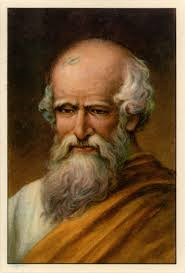
\includegraphics[width=0.2\textwidth]{pictures/archimedes.png}
\caption{Archimedes}
\end{figure}
\begin{flushleft}
Mathematica efficiunt virtutes arcanas, quas nemo intelligit, et quas ignara pulchritudinis agnitio partem habere debet. Ex infinitate consiliorum mathematicus unam formam eligit pulchritudinis causa et eam ad terram deducit.
\end{flushleft}

\begin{enumerate}
\item Here we are able to begin with a formula $e^{i\pi}+1=0$.

$$ e=\lim_{n\to\infty}\left(1+\frac{1}{n}\right)^n = \lim_{n\to\infty}\frac{n}{\sqrt[n]{n!}}$$


    \item we can also do:

$$ e=\sum_{n=0}{\infty} \frac{1}{n!}$$
    \item here we can do another:
$$ e=2+\frac{1}{1+\frac{1}{2+\frac{2}{3+\frac{3}{4+\frac{4}{5+\ddots}}}}} $$
\end{enumerate}
\pagebreak
\begin{flushleft}
Table~\ref{tab:formulas} Mathematical formulas in table
\end{flushleft}
\begin{table}[htbp]
\centering
\begin{tabular}{|l|l|l|l|l|l|}
\hline
\rowcolor[HTML]{F9522E}
Harmonic & Period & frequency(cycle/samp.int.) & frequency (rad/samp.int.) \\ \hline
1 & n & 1/n & $2\pi/n$ \\ \hline
2 & n/2 & 2/n & $4\pi/n$ \\ \hline
3 & n/3 & 3/n & $6\pi/n$ \\ \hline
$\ddot$ & $\ddot$ & $\ddot$ & $\ddot$ \\ \hline %i have some kind of problem in this line and i couldn’t find it
$n/2-1$ & $n/(n/2-1)$ & $(n/2-1)/n$ & $(n-2)\pi/n$ \\ \hline
n/2 & 2 & 1/n & $\pi$
\end{tabular}
\label{tab:formulas}
\caption{Caption of my table is below it.}
\end{table}
%and the ending of the table is not finished idk why???